% Ch2LiteratureReview.tex

\chapter[Literature Review]{Literature Review}
\label{cha:cha2LiteratureReview}

This chapter reviews the extant literature on frog call classification. 
It aims to give a quantitative and detailed analysis of related techniques used in frog call classification. Since previous studies have not used multiple-instance multiple-label (ML) learning or multiple-label (ML) learning for frog call classification, we just focus on the studies of single-instance single-label (MIML) classification of frog calls.    

\section{Introduction}
\label{intro}
Over the past decade, frog biodiversity has rapidly declined because of frogs' sensitive to habitat loss and degradation, introduced invasive species, and environmental pollution \citep{dudgeon2006freshwater}. On one hand, frog biodiversity is rapidly declining, and on the other frogs are greatly valuable for the environment. Firstly, frogs are an integral part of the food web, and the decline of their population can result in negative impacts through the whole ecosystem. Secondly, frogs are famous indicator species for environment health. Finally, frogs are very useful in medical research that benefit human \footnote{http://www.savethefrogs.com/why-frogs}. The rapid biodiversity decline and great importance of frogs make it necessary for frog biodiversity monitoring to increase. 

To monitor the change of frog biodiversity and optimise the protection policy, many researchers have shown interest in studying frogs. Compared to counting frogs by visual observation, hearing the vocalisations of frogs is much easier. Consequently, frog vocalisations are often used for monitoring frogs. There are two approaches for acoustic frog monitoring. The traditional field survey methods require ecologists to physically visit sites to collect acoustic data, which are both time-consuming and costly. In contrast, recent advances in acoustic sensor techniques have greatly extended the spatio-temporal scale for acoustic monitoring of frog biodiversity \citep{wimmer2013analysing}. The large volumes of acoustic data collected this way make it essential to develop new automated methods of analysis. 


Over the last few years, many researchers have described automated methods for detecting and classifying frog calls \citep{huang2008realization, huang2009frog, han2011acoustic,chen2012automatic, Gingras2013, camacho2013automatic, Huang20141, Xie1504:Acoustic}. However, there is no paper that summarises those methods. In this work, we present a comprehensive survey of frog call classification to provide acoustic signal researchers with basic information, current methods and trends in this field. 

Three parts play important roles in the performance and precision of frog call classification: signal pre-processing, feature extraction, and classification. In this survey, these three important parts of frog call classification are presented as shown in Fig.~\ref{fig:flowchart}. 


Signal pre-processing consists of signal processing, noise reduction and syllable segmentation. Signal processing often denotes changing a signal from one-dimension (audio data) into two-dimensional representation (image). Noise reduction is essential to improve the classification performance. Since the elementary acoustic unit for frog call classification is the syllable, which is a continuous vocalization emitted by an individual, segmenting continuous recordings of frog calls into individual syllables is necessary. 

Previous studies have developed various methods for feature extraction \citep{huang2008realization, huang2009frog, han2011acoustic, chen2012automatic, Gingras2013, camacho2013automatic, Huang20141, Xie1504:Acoustic}. Here we review and analyse all the used features: time domain and frequency domain features, 
time-frequency features, cepstral features, and other features. After feature extraction, numerous classifiers have been proposed for frog call classification. A summary of those classifiers is given in section \ref{classifiers}.


It is worth noting that most previous researchers used different databases for their experiments because frog call research is often related to geographical regions \citep{jang2011geographic}. Consequently, there is still a lack of uniformity in the way classification methods are evaluated and assessed. This survey is not meant to compare all previous frog call classification methods and find the best one, but to assemble all the methods to provide other researchers with a direction for the classification of frog calls. To be specific, we mainly survey different features used for frog call classification because most studies focus on new features rather than new signal processing techniques, syllable segmentation methods, or classifiers.

%\begin{figure*}[htb!]
%\centering
%    \begin{subfigure}[b]{\textwidth}
%           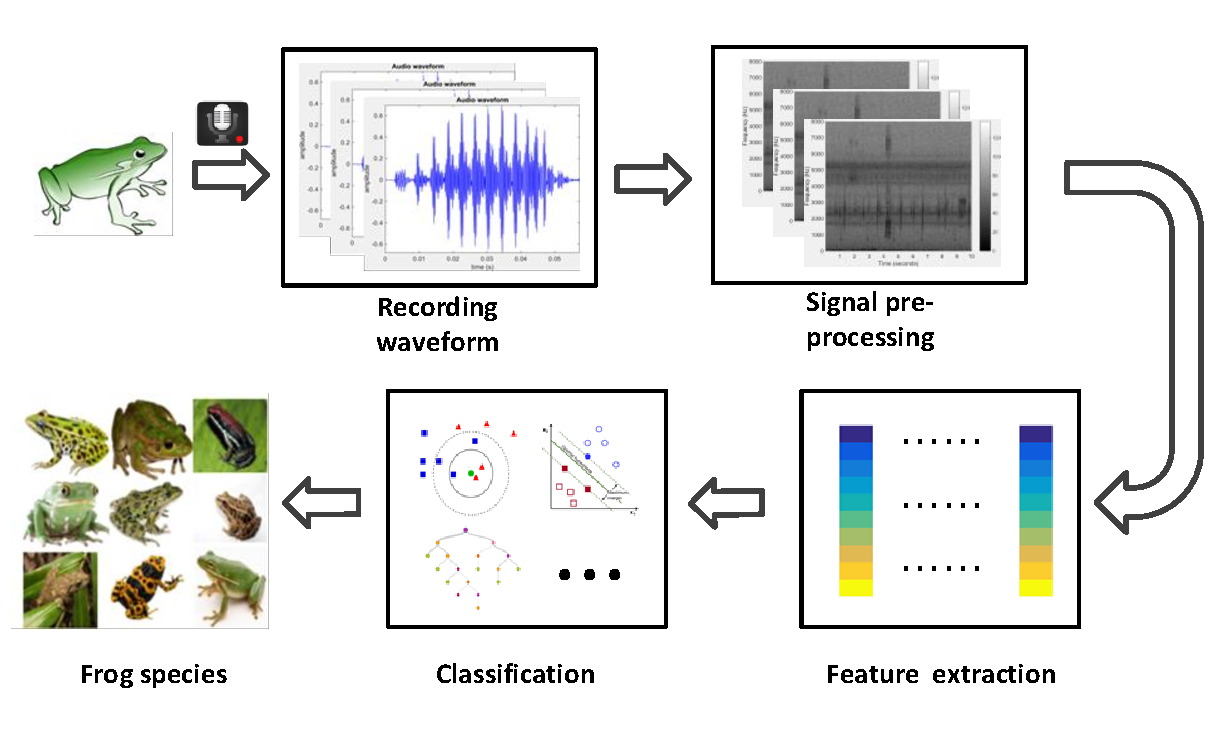
\includegraphics[width=\textwidth]{image/flowchart.pdf}
%    \end{subfigure}%
%\caption{Flowchart of frog call classification: pre-processing, feature extraction, and classification.}
%\label{fig:flowchart}       
%\end{figure*}


The remainder of this survey is organised as follows: In section \ref{pre-processing}, signal pre-processing is presented in its three parts: signal processing, noise reduction, and syllable segmentation. 
In section \ref{features}, different acoustic features are investigated for frog call classification. In section \ref{classifiers}, numerous classifiers are studied for frog call classification. In section \ref{experiment}, experimental results of state-of-the-art research are discussed. Finally, the discussion and conclusion are given in sections \ref{discussion} and \ref{conclusion}, respectively.




\section{Signal pre-processing}
\label{pre-processing}

For frog call classification, signal pre-processing is the first step after acoustic data is collected. It often consists of signal processing, noise reduction, and syllable segmentation. Each part of signal pre-processing is described below.


\subsection{Signal processing}
Signal processing often denotes the transformation of frog calls from one-dimension (recording waveform) to two dimensions (time-frequency representation). Many techniques have been developed for this transformation including short-time Fourier transform (STFT) \citep{STFT1977}, Wigner-Ville distribution \citep{WV1987}, and wavelet transform \citep{meyer1995wavelets}. STFT is the most widely used technique among them for its flexible implementation and better applicability. Given one frog call $x(t)$, its fast Fourier transform can be expressed as
\begin{equation}
X(k) = \sum_{n=0}^{L-1}x(n)w(n)e^{-j2 \pi kn/L}, 0 \leq k \leq L-1
\end{equation}
where $X(k)$ is the frequency domain signal (spectrum) and denotes each frame of the spectrogram, and $w(n)$ is the window function. The waveform, spectrum and spectrogram of one individual syllable for \textit{Mixophyes fasciolatus} is illustrated in Fig.~\ref{fig:spectrogram}. Here three representations are consistent with features in three domains: the time domain, frequency domain and time-frequency domain.

\begin{figure*}[htb!]
\centering
      \begin{subfigure}[b]{0.32\textwidth}
           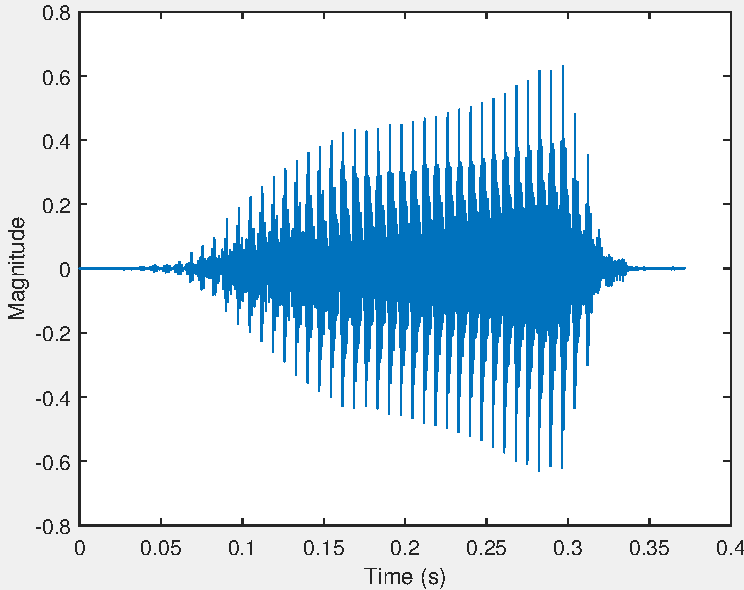
\includegraphics[width=1\textwidth,height=0.75\textwidth]{image/LR/waveform.pdf}
    \end{subfigure}%
	~
	      \begin{subfigure}[b]{0.32\textwidth}
           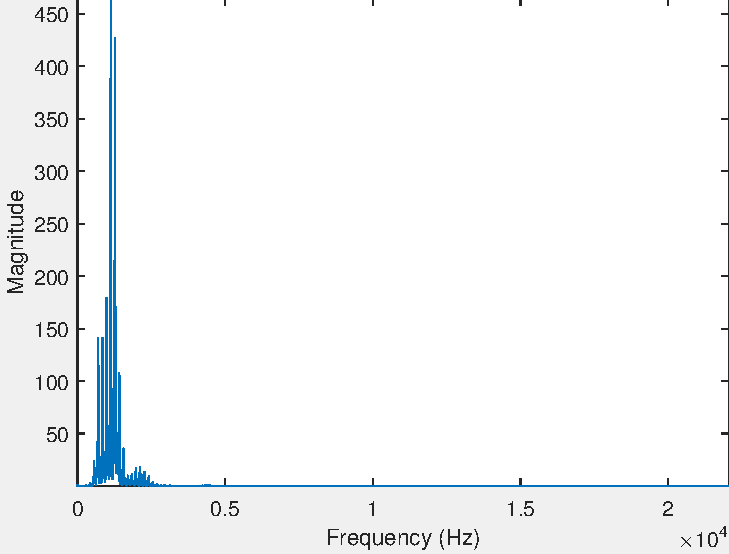
\includegraphics[width=1\textwidth,height=0.75\textwidth]{image/LR/spectrum.pdf}
    \end{subfigure}%
	~
    \begin{subfigure}[b]{0.32\textwidth}
           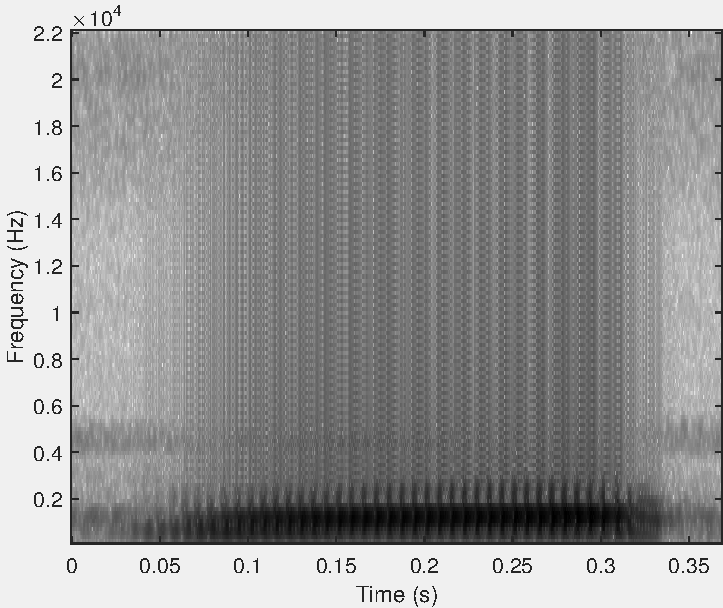
\includegraphics[width=1\textwidth,height=0.75\textwidth]{image/LR/spectrogram.pdf}
    \end{subfigure}%
\caption[Waveform, spectrum and spectrogram of one frog syllable]{Waveform, spectrum and spectrogram of one frog syllable for \textit{Mixophyes fasciolatus}. The window function, size and overlap are Hamming window, 128 samples and 85\%, respectively}
\label{fig:spectrogram}       % Give a unique label
\end{figure*}


%So far, wavelet packet decomposition (WPD) is the another technique that applied for frog call classification \citep{jie2015escience}. However, different from 

%Besides STFT, Xie et al recently introduced . 
%Compared with STFT, WPD has a better frequency resolution.


\subsection{Noise reduction}
Noise reduction is an optional process for frog call classification. 
\cite{Huang20141} applied a de-noise filter for noise reduction. The wavelet threshold function in the one-dimensional signal was used as the filter kernel function.
\cite{bedoya2014automatic} introduced spectral noise gating method for noise reduction. Specifically, the selected frequency band spectrum of the frogs' call to be detected was estimated and suppressed. \cite{emr2015Xie} used Wiener filtering to remove the background graininess, then applied spectral subtraction to the filtered spectrogram using a modified method from the adaptive level equalization algorithm. While the aforementioned noise reduction methods can remove some background noise, some of the desired signals will be suppressed. Noise reduction methods are therefore selectively used based on signal-to-noise ratio of the acoustic data and the research problem.




\subsection{Syllable segmentation}
For frog calls, the basic elementary acoustic unit is a syllable, which is a continuous frog vocalisation emitted by an individual frog \citep{huang2009frog}. The precision of syllable segmentation will directly affect the classification performance, since features used for frog call classification are calculated based on each syllable. Frog syllable segmentation methods in previous studies are summarised and listed in Table \ref{tab:segmentation}. All previous methods except \citep{jie2015ICIP} cannot address recordings with simultaneous vocalising frog calls. Meanwhile, those methods that used the time domain feature for segmentation, cannot address recordings with low signal-to-noise ratio. \cite{jie2015ICIP} introduced an unsupervised learning method, which included multiple image processing techniques for syllable segmentation. However, the downside of this unsupervised process was that not all segmented syllables correspond to frog vocalisations.

%Since the accuracy of segmentation results directly affect the final classification accuracy \citep{Colonna20157367}, meanwhile we focus on the evaluation of different features for frog call classification in this survey, we manually segment the frog calls for reducing the effect of segmentation result for classification accuracy,
  
\begin{table}[htb!]
\centering
\caption[Summary of related work]{Summary of related work for frog syllable segmentation. Here, E denotes energy, ZCR denotes zero-crossing rate.}
\label{tab:segmentation}
\resizebox{\textwidth}{!}{
\begin{tabular}{lll}
\hline\hline
{\bf Authors} & {\bf Features for segmentation}                    & {\bf Procedure}                          \\ \hline
   \citet{han2011acoustic}            & Spectral entropy                  & Manual                                      \\ 
  \citet{jaafar2013}             & E and ZCR                         & Sequential                \\ 
    \citet{huang2009frog}           & Amplitude                         & Non-sequential                           \\ 
    \citet{chen2012automatic}           & Spectrogram                         & Non-sequential            \\ 
     \citet{Xie1504:Acoustic}          & Spectrogram                       & Non-sequential           \\ 
     \citet{Colonna20157367}          & Incremental E and Incremental ZCR & Sequential and real time      \\
     \citet{jie2015ICIP}   &    Image processing    & Non-sequential    \\    
      \hline\hline
\end{tabular}
}
\end{table}




\section{Acoustic features for frog call classification}
\label{features}
Developing effective acoustic features that show greater variation between rather than within species is important for achieving robust classification results \citep{Fox20081187}. For frog call classification, acoustic features can be classified into four categories: time domain and frequency domain features, time-frequency domain features, cepstral features, and other features. 

\subsection{Time domain and frequency domain features for frog call classification}

Time domain features for frog call classification have been explored for a long time \citep{huang2008realization, huang2009frog, dayou2011classification, chen2012automatic, camacho2013automatic, Huang20141}. Time domain features are often combined with frequency domain features for frog call classification.
 
\cite{huang2009frog} used spectral centroid, signal bandwidth, and threshold-crossing rate for frog call classification with a k-nearest neighbour classifier (K-NN) and support vector machines (SVM). In another work, \cite{Huang20141} combined spectral centroid, signal bandwidth, spectral roll-off, threshold-crossing rate, spectral flatness, and average energy to classify frog calls using neural networks. Another paper published by  \citep{huang2008realization} used spectral centroid, signal bandwidth, spectral roll-off, and threshold-crossing rate for frog call classification. 
\cite{dayou2011classification} combined Shannon entropy, R$\acute{e}$nyi entropy and Tsallis entropy for frog call classification. Based on this work,  \cite{han2011acoustic} improved the classification accuracy by replacing Tsallis entropy with spectral centroid.
To classify anurans into four genera, a three-parameter model was proposed based on advertisement calls, \footnote[1]{an advertisement call is produced by a male frog in order to attract females during the breeding season and to warn other rival males of his presence.} which used mean values for dominant frequency, coefficients of variation of root-mean square energy, and spectral flux \citep{Gingras2013}. With this model, three classifiers  were employed for classification: K-NN, a multivariate Gaussian distribution model and a Gaussian Mixture Model (GMM) \citep{Gingras2013}.
\cite{chen2012automatic} proposed a method based on syllable duration and a multi-stage average spectrum for frog call recognition. Their recognition stage was completed by the Euclidean distance-based similarity measure. \cite{camacho2013automatic} used the loudness, timbre and pitch to detect frogs with a multivariate ANOVA test.






\subsection{Time-frequency features for frog call classification}

For frog call classification, we often transform the one-dimensional signal into its two-dimensional time-frequency representation. Then features based on the time-frequency representation can be calculated for classification.
\cite{acevedo2009automated} developed two feature sets for automated animal classification. The first was minimum and maximum frequencies, call duration, and maximum power; the second was minimum and maximum frequencies, call duration, and frequency of maximum power in eight segments of duration. With two feature sets, three classifiers were used for the classification: linear discriminant analysis(LDA), decision tree and SVM. \cite{brandes2008feature} proposed a method for classifying animals using duration, maximum frequency, and frequency bandwidth, and with Hidden Markov Model (HMM) used as the classifier.  \cite{yen2002automatic} combined wavelet packet feature extraction and two different dimensionality reduction algorithms to produce the final feature vectors. Then, they adopted a neural network classier for classification. \cite{grigg1996monitoring} developed a system to monitor the effect on frog population of Queensland of the introduced Cane Toad. The classification was based on the local peaks in the spectrogram using Quinlan's machine learning system, C4.5. \cite{Brandes2006} proposed a method to classify frogs using central frequency, duration, and bandwidth with a Bayesian classifier. \cite{croker2012using} introduced a feature vector for detecting frogs with a similarity measure based on Euclidean distance. The feature vector consisted of dominant frequency, frequency difference between the lowest and dominant frequencies, frequency difference between the highest and dominant frequencies, time from the start of the sound to the peak volume, and time from the peak volume to the end of the sound. \cite{Xie1504:Acoustic} developed a method for frog call classification using syllable duration, dominant frequency, oscillation rate \footnote{Oscillation rate denotes the
number of pulses within one second.}, frequency modulation, and energy modulation using a K-NN classifier. 
 


\subsection{Cepstral features for frog call classification}

Cepstral features are also popular for frog call classification. These features include Linear Prediction Coefficients (LPCs), Mel-frequency cepstral coefficients (MFCCs), and perceptual wavelet packet decomposition sub-band cepstral coefficients (PWSCCs) \citep{jie2015escience}. 
\cite{colombia2009frogs} introduced LPCs for frog call classification with a modified K-Means classifier. \cite{jaafarcomparative} introduced MFCCs and LPCs as features, and K-NN and SVM as classifiers for frog call identification. \cite{yuan2012frog} also used MFCCs and LPCs as features, and K-NN as the classifier for frog sound identification.
\cite{lee2006automatic} used the averaged MFCCs and LDA for the automatic recognition of animal sounds. \cite{bedoya2014automatic} combined MFCCs and a learning algorithm for multivariate data analysis (LAMDA) for frog call recognition. \cite{vaca2010using} proposed a method to identify animal species, which consisted of MFCCs, principal component analysis (PCA) and K-NN. \cite{jaafar2013, jaafar2013mfcc, tanintelligent2014} published three papers about frog call classification with MFCCs, $\Delta$ MFCC and $\Delta \Delta$ MFCC calculated as features, and K-NN and SVM used as classifiers. \cite{feature2012Colona} introduced MFCCs for classifying anurans with a K-NN classifier.
\cite{jie2015escience} proposed a novel feature set named perceptual wavelet packet decomposition sub-band cepstral coefficients for frog call classification. Compared with MFCCs, this feature set was more suitable for the frequency distribution of frog calls and provided a better performance for classifying frog calls . \cite{Noda2016100} fused time domain features with cepstral features for frog call classification which achieved a better classification performance than using only cepstral features. Three classifiers were investigated for the classification: HMM, random forest, and SVM.


\subsection{Other features for frog call classification}
Besides time domain features, frequency domain features, time-frequency domain features and cepstral features, other features are also introduced to classify frog calls.
\cite{wei2012distributed} proposed a distributed sparse approximation method based on $\ell 1$ minimization for frog call classification. \cite{dang2008lightweight} extracted vocalization waveform envelope as features, then classified calls by matching the extracted envelope with the original signal envelope.  \cite{emr2015Xie} used two feature sets for frog call classification: (1) minimum frequency, maximum frequency, bandwidth, duration, acoustic event area, acoustic event perimeter, acoustic event non-compactness, acoustic event rectangularity. (2) frequency mean, frequency variance, frequency skewness, frequency kurtosis, time mean, time variance, time skewness, time kurtosis, mask mean, mask standard deviation. Feature set (1) was used to describe the mask of each segmented event, feature set (2) was used to describe the statistical properties of each segmented event, each event corresponds to an individual event in 
Fig. \ref{fig:evenets}. Meanwhile, \cite{jie2015ICIP} introduced ridge related features for frog call classification: mean value for dominant frequency, low and high frequencies, histogram of ridges, and entropy of ridges in horizontal and vertical directions.




\begin{figure}[htb!]
\centering
      \begin{subfigure}[b]{0.5\textwidth}
           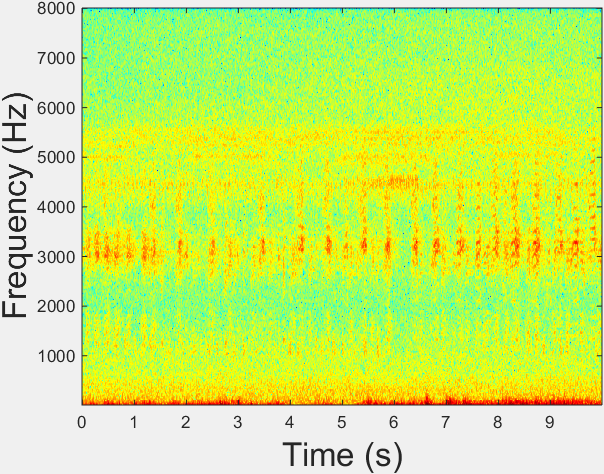
\includegraphics[width=1\textwidth,height=0.75\textwidth]{image/LR/spectrogram.png}
    \end{subfigure}%
	~~
	      \begin{subfigure}[b]{0.5\textwidth}
           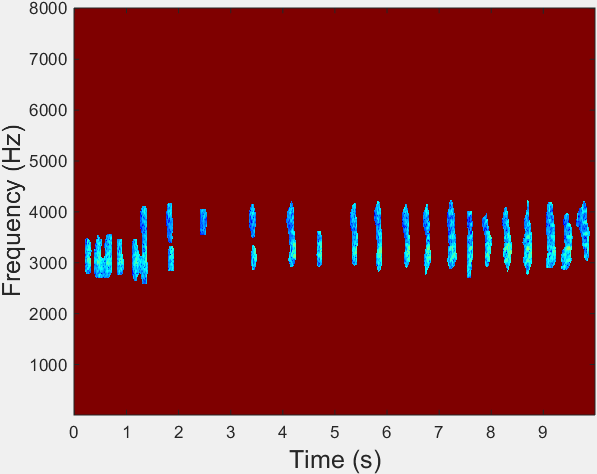
\includegraphics[width=1\textwidth,height=0.75\textwidth]{image/LR/segmentEvents.png}
    \end{subfigure}%
\caption[Acoustic event detection]{Original spectrogram and segmented events after applying acoustic event detection to the original spectrogram image.}
\label{fig:evenets}       % Give a unique label
\end{figure}



\section{Classifiers}
\label{classifiers}
For frog call classification, numerous pattern recognition methods have been used to construct the classifier, such as the Bayesian classifier \citep{Brandes2006}, k-nearest neighbour classifier (K-NN) \citep{ huang2008realization,huang2009frog, han2011acoustic, dayou2011classification, jaafar2013, Gingras2013, jaafar2013mfcc,jaafarcomparative, yuan2012frog, vaca2010using, Xie1504:Acoustic, emr2015Xie, jie2015escience, feature2012Colona}, support vector machine (SVM) \citep{huang2008realization,acevedo2009automated, huang2009frog, tanintelligent2014, Gingras2013,jaafarcomparative,jie2015ICIP}, hidden Markov model (HMM) \citep{brandes2008feature}, Gaussian mixture model (GMM) \citep{huang2008realization, Gingras2013}, neural networks (NN) \citep{Huang20141, yen2002automatic}, decision tree (DT) \citep{grigg1996monitoring, acevedo2009automated}, one-way multivariate ANOVA \citep{camacho2013automatic}, and linear discriminant analysis (LDA) \citep{acevedo2009automated,lee2006automatic}.  Besides classifiers, other methods for classifying frog species include those based on the similarity measure \citep{croker2012using, dang2008lightweight, chen2012automatic} and those based on the clustering technique \citep{colombia2009frogs, wei2012distributed, bedoya2014automatic}. K-NN is the most commonly used classifier for its simplicity and easy application. However, the K-NN classifier is sensitive to the local structure of the data, as well as to the initial cluster centroids. Therefore, the K-NN classifier is often run multiple times based on different initial points. 
SVM is another classifier which is widely used for its good generalization ability. However, the performance of SVM can be quite sensitive to the selection of the regularization and kernel parameters, and it is possible to over-fit when tuning these hyper-parameters. Therefore, selecting suitable parameters for SVM is very important and is realized by grid search in most previous studies  \citep{hsu2003practical}.



\section{Experiment results of the state-of-the-art methods}
\label{experiment}


\subsection{Evaluation criteria}

Accuracy is the most widely used statistical criterion for evaluating frog call classification. Other evaluation criteria such as precision, recall, sensitivity, specificity, F-measure, and ROC curves are also used. Before defining these evaluation criteria, we first define true positives (TP), true negatives (TN), false negatives (FN), and false positives (FP) as described by  \citep{gordon2003sequence} 
(1) TP: correctly recognized positives;
(2) TN: correctly recognized negatives;
(3) FN: positives recognized as negatives;
(4) FP: negatives recognized as positives.
Then, accuracy, precision, recall (sensitivity), and specificity can be defined as follows.

\begin{equation}
Accuracy = \frac{TP+TN}{TP+TN+FP+FN}
\end{equation}

\begin{equation}
Precision = \frac{TP}{TP+FP}
\end{equation}

\begin{equation}
Recall = \frac{TP}{TP+FN}
\end{equation}

\begin{equation}
Specificity = \frac{TN}{FP+TN}
\end{equation}


\subsection{Experiment results for summarise}


Table \ref{tab:classificationPerformance} shows the list of summarised frog call classification methods, together with the database they used and corresponding performance.



\begin{table}[htb!]
\centering
\caption[Overview of frog call classification performance]{A brief overview of frog call classification performance. The asterisk denotes that frog species are not the only animal species to be studied.}
\label{tab:classificationPerformance}
\resizebox{\textwidth}{!}{
\Rotatebox{90}{%
\begin{tabular}{llll}
\hline\hline
\textbf{Database}                   & \textbf{Performance}                   & \textbf{Reference} & \textbf{Data source} \\ \hline
3 frog species with 635 calls & Precision of 99\%, recall of 92\% & \citet{camacho2013automatic} &  Collected from Costa Rica (unavailable)     \\ 
1 frog species with 100 samples   & \begin{tabular}[c]{@{}l@{}}Sensitivity of 0.85 with specificity of 0.92  \\ when distinguishing \textit{Mixophyes iteratus} calls from \\ other species' call. Sensitivity of 0.88 with \\ specificity   of 0.82 against background noise \end{tabular}  & \citet{croker2012using} &  Recorded next to a running stream (unavailable) \\ 
17 animal types & \begin{tabular}[c]{@{}l@{}}  50\% true positive accuracy, \\ over 50\ false-negative for 4 animal types \end{tabular}  & \citet{Brandes2006} & Collected from NE Costa Rica (unavailable) 
\\   
22 frog species &  NA  & \citet{grigg1996monitoring} & Collected from Queensland, Australia (unavailable) \\ 
4 frog species with 66 samples & \begin{tabular}[c]{@{}l@{}}  Best performance with averaged classification \\ Accuracy of 72.18\% and 0.76\% for standard \\ deviation.  \end{tabular}  &  \citet{yen2002automatic} & Unknown \\
\begin{tabular}[c]{@{}l@{}} 10 frog species, 9 bird species, \\ and 8 cricket species \end{tabular} & Accuracy of 88\% for frogs    & \citet{brandes2008feature}* & Collected from NE Costa Rica (unavailable) \\ 
\begin{tabular}[c]{@{}l@{}} 9 frog species and 3 bird species \\ with 10061 samples \end{tabular} & \begin{tabular}[c]{@{}l@{}} Best true positive rate of 94.95\% and \\ 0.94\% for false positive rate \end{tabular} &  \citet{acevedo2009automated}* &   Collected from 14 montane sites in Puerto Rico
 \\  
9 frog species with 90 syllables &  Averaged classification accuracy of 90.00\%      &  \citet{dayou2011classification}  &   Obtained from http://www.Frogsaustralia.
net.au/frogs \\ 

  9 frog species with 54 syllables   & Averaged classification accuracy of 98.00\%  &   \citet{han2011acoustic} &   Obtained from http://www.Frogsaustralia.
net.au/frogs \\ 

5 frog species with 727 syllables & Averaged classification accuracy of 95.86\%     &   \citet{huang2008realization}  & Unknown  \\ 

142 species belonging to four genera   &  Genus classification accuracy above 70\%    &     \citet{Gingras2013} & obtained from
commercially available compact discs (CDs) (available)  \\ 

18 frog species with 960 syllables & Classification accuracy of 94.3\%   &   \citet{chen2012automatic} & \begin{tabular}[c]{@{}l@{}} Recorded in a wild field located in \\ the Shan-Ping forest ecological garden in Kaohsiung city, \\ Taiwan (unavailable) \end{tabular} \\ 

13 frog species with 1514 samples &  Averaged recognition rate of 93.4\%    &    \citet{Huang20141}  &   Unknown \\ 

5 frog species with 959 samples      &   Averaged classification accuracy of 90.03\%       &    \citet{huang2009frog}  &   Unknown        \\ 

15 frog species with 286 samples &       Averaged classification accuracy of 95.67\%   &  \citet{tanintelligent2014} & recorded at Sungai Sedim, in Kulim, Kedah, Malaysia   \\ 
8 frog species with 160 samples & averaged classification accuracy of 98.1\%        &  \citet{yuan2012frog} &  Obtained from AmphibiaWeb (http://amphibiaweb.org/)(available)
\\ 
10 frog species with 250 syllables   &       Averaged classification accuracy of 98.8\%   &  \citet{jaafarcomparative} & \begin{tabular}[c]{@{}l@{}} Internet database (http://learning.froghome.org/) \\ and IBM,USM (http://www.frogwatch.org.au/?action=animal.list) (available) \end{tabular}  \\ 

15 frog species with 386 syllables  &    Averaged classification accuracy of 85.78\%   &   \citet{jaafar2013mfcc} & Recorded from locations around Baling
and Kulim, Kedah, Malaysia (unavailable)
 \\ 
12 frog species with 291 syllables &   Averaged classification accuracy of 97\%   & \citet{jaafar2013}  & Recorded from locations around Baling
and Kulim, Kedah, Malaysia (unavailable)
\\  
\begin{tabular}[c]{@{}l@{}} 12 frog species with 379 samples,  \end{tabular}  \\ 10 bird species with 193 samples &  Averaged classification accuracy of 86.6\%    &   \citet{vaca2010using} &   \begin{tabular}[c]{@{}l@{}} Recorded in Puerto Rico  (http://www.amazon.com/Los\\-Anfibios-Reptiles-Puerto-Rico/dp/084770243X) (available) \end{tabular} 
 \\ 
13 frog species with 916 calls & \begin{tabular}[c]{@{}l@{}} Averaged classification accuracy of 100\%, \\ and 99.61\% respectively for two database \end{tabular}  &  \citet{bedoya2014automatic}  &  \begin{tabular}[c]{@{}l@{}} Provided
by the Smithsonian Tropical Research Institute (STRI) \\ and the Grupo Herpetológico de Antioquia (GHA) (unavailable) \end{tabular}   \\ 
30 frog species and 19 cricket calls  &  \begin{tabular}[c]{@{}l@{}}  Averaged classification accuracy of 96.8\% \\ and 98.1\% \end{tabular}  & \citet{lee2006automatic}  & Derived from compact disk (unavailable) \\ 


15 frog species with 896 syllables   & Precision of 99.00\%  &   \citet{Colonna20157367} & Obtained from Internet(http://
bit.ly/1b8bvyE) (available)  \\ 

10 frog species with 516 syllables & Averaged classification accuracy of 97.45\%    & \citet{jie2015escience}  &  Collected from compact disk (http://www.naturesound.com.au/) (available) \\

  15 frog species with 436 syllables             &        Averaged classification accuracy of 74.73\%         &      \citet{jie2015ICIP}  &  Collected from compact disk (http://www.naturesound.com.au/) (available)  \\ 

16 frog species with 898 syllables    & Averaged classification accuracy of 90.5\%   &    \citet{Xie1504:Acoustic}  &  Collected from compact disk (http://www.naturesound.com.au/) (available)       \\ 

 14 frog species with 985 syllables & Averaged classification accuracy of 87.00\%   &    \citet{emr2015Xie}    &   \begin{tabular}[c]{@{}l@{}} Collected from compact disk (http://www.naturesound.com.au/) (available) \\ and one public website (http://amphibiaweb.org/maps/index.html) \end{tabular}    \\ 

  9 frog species with 49 samples            &    Averaged classification accuracy of 97.60\%  & \citet{feature2012Colona} &  \begin{tabular}[c]{@{}l@{}} Collected on the campus of the Federal
University of Amazonas in \\ Manaus, Brazil (unavailable) \end{tabular} 
\\ 

3 frog species with 50 samples &  Averaged  classification accuracy of 90\%       &           \citet{dang2008lightweight} & Unknown \\

\begin{tabular}[c]{@{}l@{}} 1564 syllables of 41 anurans, \\ 5201 syllables of 58 frogs, \\ 10905 syllables of 100 anurans, \\ and 17671 syllables of 199 anurans \end{tabular} & 98.8\%, 96.9\%, 95.48\%, and 95.38\% respectively  & \citet{Noda2016100}  & \begin{tabular}[c]{@{}l@{}}  AmphibiaWeb(41 anurans), 58 frogs from Cuba, \\
100 anurans from Brizil-Uruguay,\\ and 199 anurans  from all datasets (http://www.nhbs.com/) (available) \end{tabular}
\\  
  
\begin{tabular}[c]{@{}l@{}}  18 frog species from commercial \\ recordings and field recordings of 8  \\ frog speciesfrom James Cook University   \\  recordings  \end{tabular} &  \begin{tabular}[c]{@{}l@{}} 99.5\% and 97.4\% for 18 frog species \\ and 8 frog species respectively   \end{tabular} &  \citet{Xie2016}  &  \begin{tabular}[c]{@{}l@{}}  David Stewart's commercial CD (http://www.naturesound.com.au/) \\ and frog calls collected from the wild (https://www.ecosounds.org/) (available) \end{tabular}
  
\\ \hline\hline
\end{tabular}
}
}
\end{table}



 
\section{Discussion and future work}
\label{discussion}
In this section, each part of a frog call classification system is discussed to give a direction for future work. 

\subsection{Database}
One major problem for frog call classification is the lack of an universal database. The databases used are often related to geographical regions, since researchers from different countries focus on particular frog species in their specific area (Table \ref{tab:classificationPerformance}). Therefore, it is difficult for researchers to compare their particular classification methods. Current studies often focus on the study of limited number of frog species (less than 100), but the number of known amphibian species is above 7000. To reach a high quality resolution, there still is a long way to go.


\subsection{Signal pre-processing}
Currently, short-time Fourier transform (STFT) is the most widely used technique for frog call classification. However, STFT has a trade-off between time and frequency resolution, which restricts the discriminability of features extracted from the spectrogram. 
In contrast, wavelet packet decomposition (WPD) has a better frequency domain resolution than STFT. The main disadvantage of WPD is the time dependence. 

Noise reduction is an optional processing step in frog call classification. For some databases of studies shown in Table \ref{tab:classificationPerformance}, frog calls have a high signal-to-noise ratio (SNR), where noise reduction is unnecessary. However, when studying recordings of low SNR, noise reduction is essential for improving the classification performance \citep{bedoya2014automatic, Huang20141}. After noise reduction, both the accuracy of syllable segmentation and feature extraction can be relatively improved.

Frog syllable segmentation based on energy and zero-crossing rate cannot address recordings with low SNR. Meanwhile, this method cannot segment recordings with overlapping frog calls. Recent use of unsupervised learning algorithms opens a path for segmenting overlapping frog syllables with image processing techniques. However, like other unsupervised algorithms, this method has the disadvantage that not all segmented syllables are frog vocalizations \citep{potamitis2015unsupervised}. Briggs et al used a supervised learning algorithm (Random Forest) for bird call segmentation. However, this method required lots of tagged acoustic data to train the classifier \citep{tjahja2015supervised}.

For syllable segmentation, time domain features are more sensitive to background noise than frequency domain features, because different frequency components can be separated by transforming the signal from time domain to frequency domain. But time domain features cannot segment those overlapping frog syllables, since time domain features have no ability to separate different frequency components. Compared to time domain features, the use of amplitude-frequency information provides a robust method to segment low SNR recordings. To address those overlapping frog syllables, image processing techniques can be a possible solution. 




\subsection{Acoustic features}
Most previous studies directly transplant features developed for speech recognition to analyze frog calls, which might not be suitable. For example, MFCCs are designed for studying speech, which are based on the calculation of a non-linear Mel-scale. However, the Mel-scale is designed for the perceptual scale of pitches judged by listeners rather than frogs. The direct use of speech features will therefore restrict classification performance. Recently, \cite{jie2015escience} used an adaptive frequency scaled wavelet packet decomposition to classify frog calls, and it achieved a better performance than Mel-scaled wavelet packet decomposition. Here, an adaptive frequency scale was generated by applying K-Means clustering to dominant frequencies, which was more accurate and efficient than using Mel-scale \citep{jie2015escience}.
Most frequency domain features are calculated by directly calculating the statistics over frames, which leads to the loss of temporal information. To add the temporal information of the feature set, time domain features can be combined with frequency domain features to achieve higher classification accuracy. Transforming audio data into its a two dimensional representation (such as a spectrogram) for quick visual analysis, has led to increasing attention being given to image processing techniques for automatically analysing animal calls. Ridges extracted from spectrogram images ware applied to perform frog call classification \citep{jie2015ICIP}. Besides ridges, other image features are worth being investigated for frog call classification.

\subsection{Classifiers}
Almost all previous studies assume that each recording has only one frog species, then a single-instance single-label classification framework is adopted to classify  frog calls. However, recent advances in acoustic sensor techniques have collected large volumes of acoustic data that have multiple simultaneously vocalising frog species, because different frog species tend to call together to make frog chorus (Figure.~\ref{fig:label}). Based on this characteristic of frog call recordings, the classification problem can be naturally framed as a multiple-instance multiple-label classification or a multiple-label classification problem rather than a single-instance single-label classification.


\begin{figure}[htb!]
\centering
    \begin{subfigure}[b]{\textwidth}
           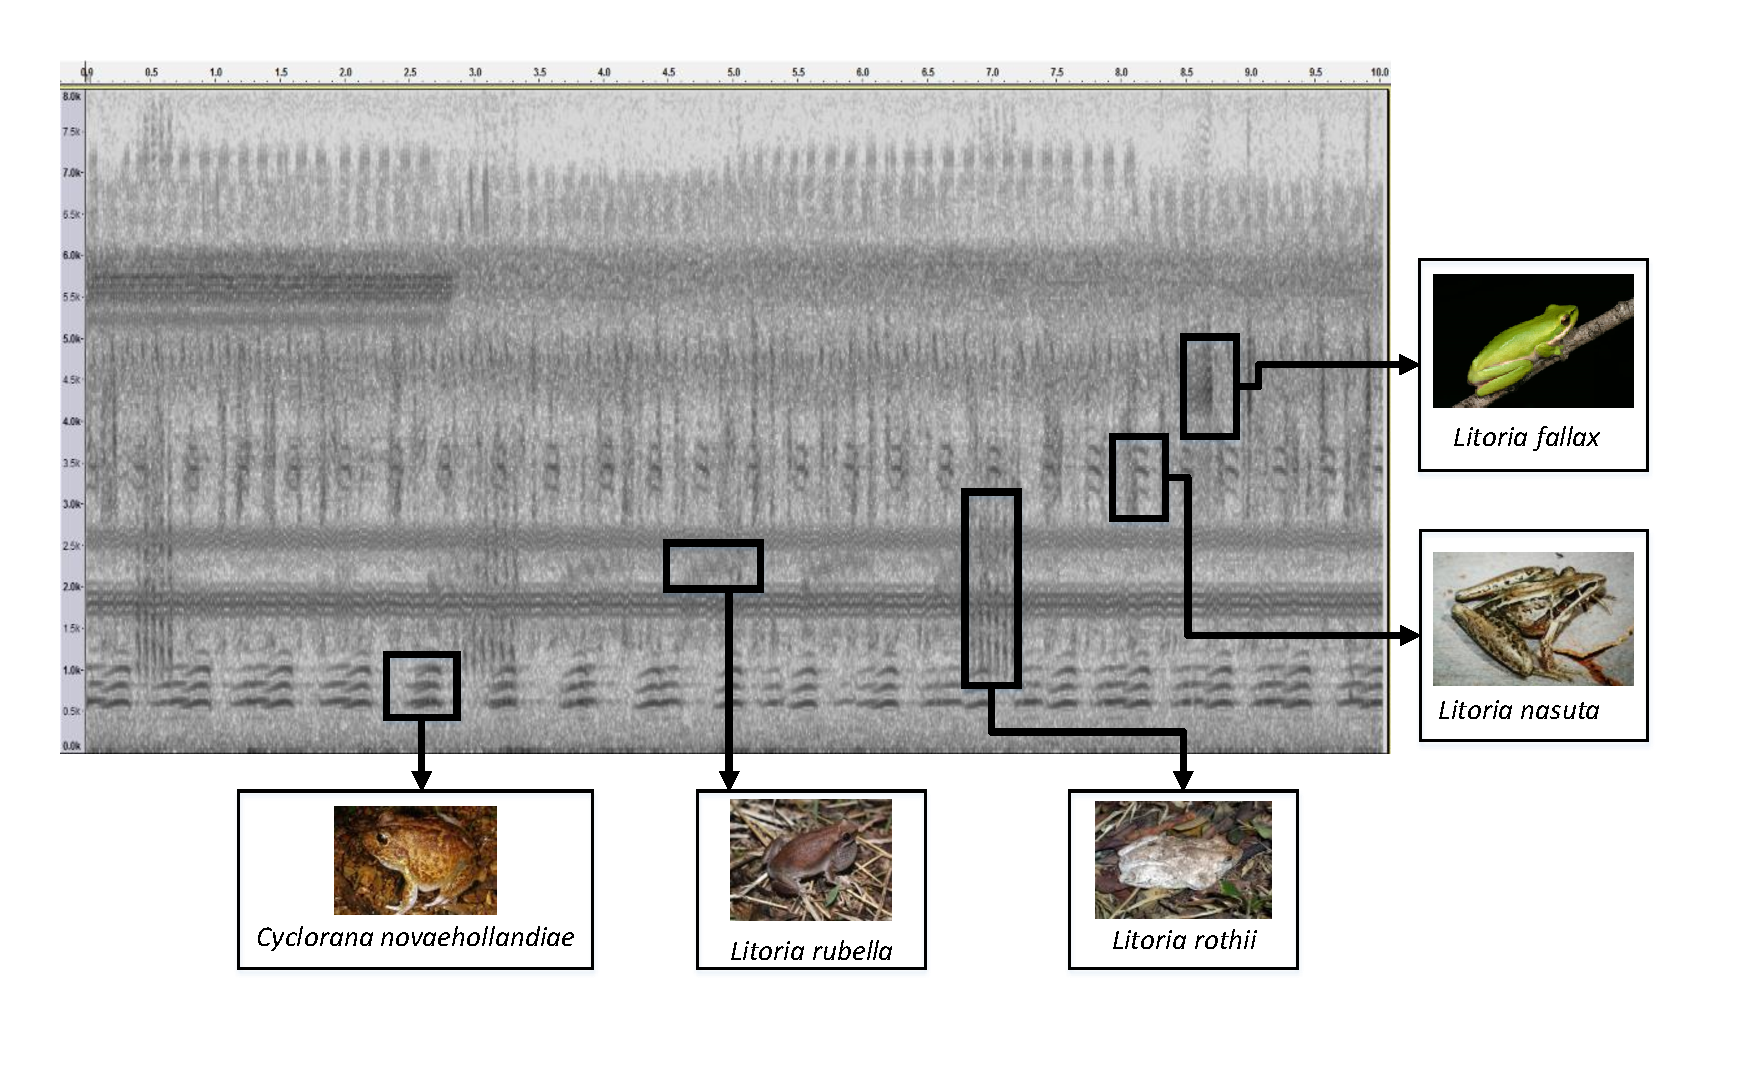
\includegraphics[width=1\textwidth]{image/LR/label.pdf}
    \end{subfigure}%
\caption[An example of collected recording]{An example of collected recording with multiple simultaneously vocalizing frog species. Five frog species exist in this 10-second recording: \textit{Cyclorana novaehollandiae}, \textit{Litoria rubella}, \textit{Litoria nasuta}, \textit{Litoria rothii}, and \textit{Litoria fallax}.}
\label{fig:label}       
\end{figure}



\section{Conclusions}
\label{conclusion}
The main objective of this survey is to provide a research direction for analysing acoustic signals, especially frog calls. With the use of signal processing and machine learning techniques, different frog species can be classified based on their vocalizations. To achieve this goal, three main parts of a frog call classification system are explained: signal pre-processing, feature extraction, and classification. For each part, current techniques used by different researchers are explored. For signal pre-processing, signal processing, noise reduction, and syllable segmentation are studied respectively. For feature extraction, acoustic features in different domains are explored. For classification, different classification frameworks are investigated: single-instance single-label classification, multi-label classification, and multi-instance multi-label classification. 

In general, frog call classification is still in its infancy as a field of study, and potential applications and unsolved problems are extending every day. For future work, it is worth further improving the accuracy and efficiency of noise reduction and syllable segmentation because they are critical processes for frog call classification. Since collected frog calls in the field often contain many background noises (birds, insects, rain, wind, human voices, etc.), it is necessary to design new noise reduction methods based on different environments. It is also necessary to develop accurate and efficient methods for syllable segmentation for its great influence in the frog call classification system performance. Currently, studies have focused on frequency domain features for classification. In the future, time domain features can be more incorporated for increasing the accuracy of frog call classification. For the classification frameworks, using MIML learning or ML learning for studying environmental recordings may be a productive research direction because of the characteristic of collected acoustic data. It is also worth making a uniform dataset that covers different frog species from different areas, since there is still no available uniform datasets of frog calls. Then researchers can evaluate their particular methods on a uniform platform.




